%%%%%%%%%%%%%%%%%%%%%%%%%%%%%%%%%%%%
% Slide options
%%%%%%%%%%%%%%%%%%%%%%%%%%%%%%%%%%%%

% Option 1: Slides with solutions

\documentclass[slidestop,compress,mathserif]{beamer}
\newcommand{\soln}[1]{\textit{#1}}
\newcommand{\solnGr}[1]{#1}

% Option 2: Handouts without solutions

%\documentclass[11pt,containsverbatim,handout]{beamer}
%\usepackage{pgfpages}
%\pgfpagesuselayout{4 on 1}[letterpaper,landscape,border shrink=5mm]
%\newcommand{\soln}[1]{ }
%\newcommand{\solnGr}{ }


%%%%%%%%%%%%%%%%%%%%%%%%%%%%%%%%%%%%
% Style
%%%%%%%%%%%%%%%%%%%%%%%%%%%%%%%%%%%%

\input{../lec_style.tex}


%%%%%%%%%%%%%%%%%%%%%%%%%%%%%%%%%%%%
% Preamble
%%%%%%%%%%%%%%%%%%%%%%%%%%%%%%%%%%%%

\title[Chp 3: Probability]{Chapter 3: Probability}
\author{OpenIntro Statistics, 4th Edition}
\institute{$\:$ \\ {\footnotesize Slides developed by Mine \c{C}etinkaya-Rundel of OpenIntro. \\
The slides may be copied, edited, and/or shared via the \webLink{http://creativecommons.org/licenses/by-sa/3.0/us/}{CC BY-SA license.} \\
Some images may be included under fair use guidelines (educational purposes).}}
\date{}

%%%%%%%%%%%%%%%%%%%%%%%%%%%%%%%%%%%%
% Begin document
%%%%%%%%%%%%%%%%%%%%%%%%%%%%%%%%%%%%

\begin{document}


%%%%%%%%%%%%%%%%%%%%%%%%%%%%%%%%%%%%
% Title page
%%%%%%%%%%%%%%%%%%%%%%%%%%%%%%%%%%%%

{
\addtocounter{framenumber}{-1} 
{\removepagenumbers 
\usebackgroundtemplate{\includegraphics[width=\paperwidth]{../OpenIntro_Grid_4_3-01.jpg}}
\begin{frame}

\hfill \includegraphics[width=20mm]{../oiLogo_highres}

\titlepage

\end{frame}
}
}


%%%%%%%%%%%%%%%%%%%%%%%%%%%%%%%%%%%%
% Sections
%%%%%%%%%%%%%%%%%%%%%%%%%%%%%%%%%%%%

%%%%%%%%%%%%%%%%%%%%%%%%%%%%%%%%%%%%

\section{Defining probability}

%%%%%%%%%%%%%%%%%%%%%%%%%%%%%%%%%%%%

\subsection{Probability}

%%%%%%%%%%%%%%%%%%%%%%%%%%%%%%%%%%%%

\begin{frame}
\frametitle{Random processes}

\twocol{0.5}{0.5}
{
\begin{itemize}

\item A \hl{random process} is a situation in which we know what outcomes could happen, but we don't know which particular outcome will happen.

\item Examples: coin tosses, die rolls, iTunes shuffle, whether the stock market goes up or down tomorrow, etc.

\item It can be helpful to model a process as random even if it is not truly random.

\end{itemize}
}{
\begin{center}
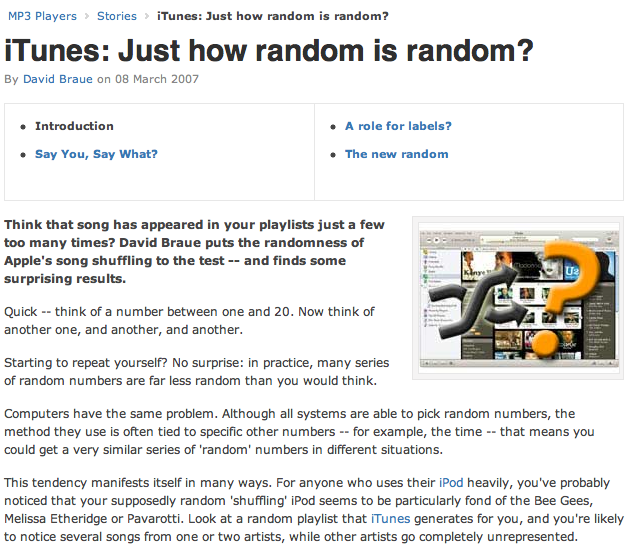
\includegraphics[width=\textwidth]{3-1_define_probability/figures/iTunes}
\end{center}
\ct{ \webURL{http://www.cnet.com.au/itunes-just-how-random-is-random-339274094.htm}}
}

\end{frame}

%%%%%%%%%%%%%%%%%%%%%%%%%%%%%%%%%%%%

\begin{frame}
\frametitle{Probability}

\begin{itemize}

\item There are several possible interpretations of probability but they (almost) completely agree on the mathematical rules probability must follow.
\begin{itemize}
\item $P(A)$ = Probability of event A 
\item $0 \le P(A) \le 1$
\end{itemize}

\pause

\item \hl{Frequentist interpretation:} 
\begin{itemize}
\item The probability of an outcome is the proportion of times the outcome would occur if we observed the random process an infinite number of times.
\end{itemize}

\pause

\item \hl{Bayesian interpretation:} 
\begin{itemize}
\item  A Bayesian interprets probability as a subjective degree of belief: For the same event, two separate people could have different viewpoints and so assign different probabilities.
\item Largely popularized by revolutionary advance in computational technology and methods during the last twenty years.
\end{itemize}

\end{itemize}

\end{frame}

%%%%%%%%%%%%%%%%%%%%%%%%%%%%%%%%%%%%

\begin{frame}
\frametitle{Practice}

\pq{Which of the following events would you be most surprised by?}

\begin{enumerate}[(a)]
\item exactly 3 heads in 10 coin flips
\item exactly 3 heads in 100 coin flips
\solnMult{exactly 3 heads in 1000 coin flips}
\end{enumerate}

\end{frame}

%%%%%%%%%%%%%%%%%%%%%%%%%%%%%%%%%%%%

\begin{frame}
\frametitle{Law of large numbers}

\hl{Law of large numbers} states that as more observations are collected, the proportion of occurrences with a particular outcome, \mathhl{\hat{p}_n}, converges to the probability of that outcome, \mathhl{p}.

\end{frame}

%%%%%%%%%%%%%%%%%%%%%%%%%%%%%%%%%%%%

\begin{frame}
\frametitle{Law of large numbers (cont.)}

\dq{When tossing a \textit{fair} coin, if heads comes up on each of the first 10 tosses, what do you think the chance is that another head will come up on the next toss? 0.5, less than 0.5, or more than 0.5?}

\[ \underline{H} \hspace{1mm} \underline{H} \hspace{1mm} \underline{H} \hspace{1mm} \underline{H} \hspace{1mm} \underline{H} \hspace{1mm} \underline{H} \hspace{1mm} \underline{H} \hspace{1mm} \underline{H} \hspace{1mm} \underline{H} \hspace{1mm} \underline{H} \hspace{1mm} \underline{?} \]

\begin{itemize}
\item<2-> The probability is still 0.5, or there is still a 50\% chance that another head will come up on the next toss.
\[ P(H \text{ on 11}^{th} \text{ toss}) = P(T \text{ on 11}^{th} \text{ toss}) = 0.5 \]
\item<3-> The coin is not ``due" for a tail.
\item<4-> The common misunderstanding of the LLN is that random processes are supposed to compensate for whatever happened in the past; this is just not true and is also called \hl{gambler's fallacy} (or \hl{law of averages}).
\end{itemize}

\end{frame}

%%%%%%%%%%%%%%%%%%%%%%%%%%%%%%%%%%%%

\subsection{Disjoint or mutually exclusive outcomes}

%%%%%%%%%%%%%%%%%%%%%%%%%%%%%%%%%%%%

\begin{frame}
\frametitle{Disjoint and non-disjoint outcomes}

\hl{Disjoint (mutually exclusive) outcomes:} Cannot happen at the same time.
\begin{itemize}
\item The outcome of a single coin toss cannot be a head and a tail.
\item A student both cannot fail and pass a class.
\item A single card drawn from a deck cannot be an ace and a queen.
\end{itemize}

\pause

\hl{Non-disjoint outcomes:} Can happen at the same time.
\begin{itemize}
\item A student can get an A in Stats and A in Econ in the same semester.
\end{itemize}

\end{frame}

%%%%%%%%%%%%%%%%%%%%%%%%%%%%%%%%%%%%

\begin{frame}
\frametitle{Union of non-disjoint events}

\dq{What is the probability of drawing a jack or a red card from a well shuffled full deck?}

\begin{figure}
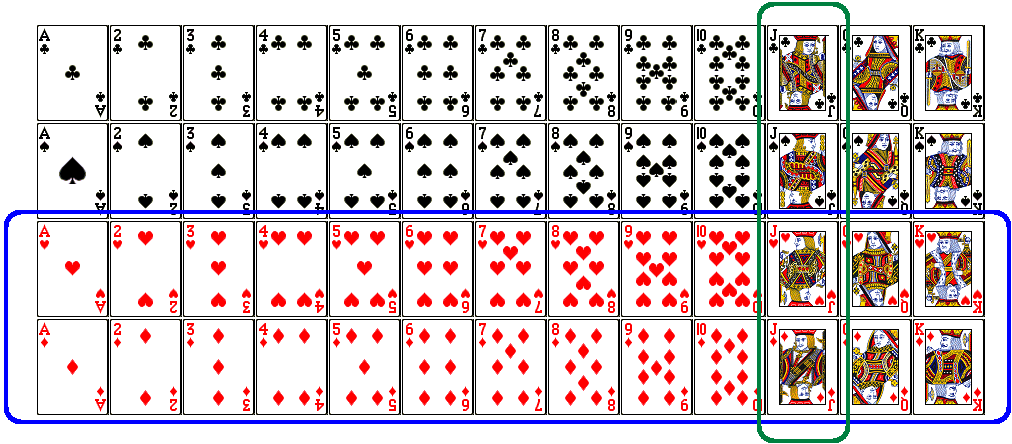
\includegraphics[width=0.7\textwidth]{3-1_define_probability/figures/cards}
\end{figure}

\vspace{-0.75cm}

\soln{\onslide<2->{
\begin{align*}
P(jack~or~red) &= P(jack) + P(red) - \orange{$P(jack~and~red)$} \\
&= \frac{4}{52} + \frac{26}{52} - \frac{2}{52} = \frac{28}{52}
\end{align*}
}}

\vfill

\ct{Figure from \webURL{http://www.milefoot.com/math/discrete/counting/cardfreq.htm}.}

\end{frame}

%%%%%%%%%%%%%%%%%%%%%%%%%%%%%%%%%%%%

\subsection{Probabilities when events are not disjoint}

%%%%%%%%%%%%%%%%%%%%%%%%%%%%%%%%%%%%

\begin{frame}
\frametitle{Practice}

\pq{What is the probability that a randomly sampled student thinks marijuana should be legalized \underline{or} they agree with their parents' political views?}

{\small
\begin{center}
\begin{tabular}{l  cc c}
            & \multicolumn{2}{c}{\textit{Share Parents' Politics}} & \\
\cline{2-3}
\textit{Legalize MJ} & No & Yes & Total \\
\hline
No          & 11 & 40 & 51 \\
Yes         & 36 & 78 & 114 \\
\hline
Total       & 47 & 118 & 165
\end{tabular}
\end{center}
}

\begin{enumerate}[(a)]
\item $\frac{40 + 36 - 78}{165}$
\solnMult{$\frac{114 + 118 - 78}{165}$}
\item $\frac{78}{165}$
\item $\frac{78}{188}$
\item $\frac{11}{47}$
\end{enumerate}

\end{frame}

%%%%%%%%%%%%%%%%%%%%%%%%%%%%%%%%%%%%

\begin{frame}
\frametitle{Recap}

\formula{General addition rule}{\[ P(A~or~B) = P(A) + P(B) - P(A~and~B) \]}

\Note{For disjoint events $P(A~and~B) = 0$, so the above formula simplifies to $P(A~or~B) = P(A) + P(B)$.}

\end{frame}

%%%%%%%%%%%%%%%%%%%%%%%%%%%%%%%%%%%%

\subsection{Probability distributions}

%%%%%%%%%%%%%%%%%%%%%%%%%%%%%%%%%%%%

\begin{frame}
\frametitle{Probability distributions}

A \hl{probability distribution} lists all possible events and the probabilities with which they occur.

\begin{itemize}
\item The probability distribution for the gender of one kid:
{\footnotesize 
\begin{center}
\begin{tabular}{r | c | c}
Event    & Male		& Female \\
\hline
Probability	& 0.5		& 0.5 \\
\end{tabular}
\end{center}
}

\pause

\item Rules for probability distributions:
\begin{enumerate}
\item The events listed must be disjoint
\item Each probability must be between 0 and 1
\item The probabilities must total 1
\end{enumerate}

\pause

\item The probability distribution for the genders of two kids:
\soln{
\only<2->{
{\footnotesize
\begin{center}
\begin{tabular}{r | c | c | c | c}
Event		& MM	& FF		& MF		& FM \\
\hline
Probability	& 0.25	& 0.25	& 0.25	& 0.25 \\
\end{tabular}
\end{center}
}}}

\end{itemize}

\end{frame}

%%%%%%%%%%%%%%%%%%%%%%%%%%%%%%%%%%%%

\begin{frame}
\frametitle{Practice}

\pq{In a survey, 52\% of respondents said they are Democrats. What is the probability that a randomly selected respondent from this sample is a Republican?}

\begin{enumerate}[(a)]
\item 0.48
\item more than 0.48
\item less than 0.48
\solnMult{cannot calculate using only the information given}
\end{enumerate}

\soln{\only<2>{\orange{If the only two political parties are Republican and Democrat, then (a) is possible. However it is also possible that some people do not affiliate with a political party or affiliate with a party other than these two. Then (c) is also possible. However (b) is definitely not possible since it would result in the total probability for the sample space being above 1.}}}

\end{frame}

%%%%%%%%%%%%%%%%%%%%%%%%%%%%%%%%%%%%

\subsection{Complement of an event}

%%%%%%%%%%%%%%%%%%%%%%%%%%%%%%%%%%%%

\begin{frame}
\frametitle{Sample space and complements}

\hl{Sample space} is the collection of all possible outcomes of a trial.

\begin{itemize}
\item A couple has one kid, what is the sample space for the gender of this kid? $S = \{ M, F \}$
\item A couple has two kids, what is the sample space for the gender of these kids? \soln{\pause{$S = \{ MM, FF, FM, MF \}$}}
\end{itemize}

\pause

\hl{Complementary events} are two mutually exclusive events whose probabilities that add up to 1.

\begin{itemize}
\item A couple has one kid. If we know that the kid is not a boy, what is gender of this kid?
\{ \sout{\textcolor{gray}{M}}, \orange{F} \} $\rightarrow$ Boy and girl are \hl{complementary} outcomes.
\item A couple has two kids, if we know that they are not both girls, what are the possible gender combinations for these kids?
\soln{\pause{\{ \orange{MM}, \sout{\textcolor{gray}{FF}}, \orange{FM}, \orange{MF} \} }}
\end{itemize}

\end{frame}

%%%%%%%%%%%%%%%%%%%%%%%%%%%%%%%%%%%%

\subsection{Independence}

%%%%%%%%%%%%%%%%%%%%%%%%%%%%%%%%%%%%

\begin{frame}
\frametitle{Independence}

Two processes are \hl{independent} if knowing the outcome of one provides no useful information about the outcome of the other.

\pause

\begin{itemize}

\item Knowing that the coin landed on a head on the first toss \underline{does not} provide any useful information for determining what the coin will land on in the second toss. $\rightarrow$ Outcomes of two tosses of a coin are independent.

\pause

\item Knowing that the first card drawn from a deck is an ace \underline{does} provide useful information for determining the probability of drawing an ace in the second draw. $\rightarrow$ Outcomes of two draws from a deck of cards (without replacement) are dependent.

\end{itemize}

\end{frame}

%%%%%%%%%%%%%%%%%%%%%%%%%%%%%%%%%%%%

\begin{frame}
\frametitle{Practice}

\pq{\small{Between January 9-12, 2013, SurveyUSA interviewed a random sample of 500 NC residents asking them whether they think widespread gun ownership protects law abiding citizens from crime, or makes society more dangerous. 58\% of all respondents said it protects citizens. 67\% of  White respondents, 28\% of Black respondents, and 64\% of Hispanic respondents shared this view. Which of the below is true?}}

Opinion on gun ownership and race ethnicity are most likely
\begin{enumerate}[(a)]
\item complementary
\item mutually exclusive
\item independent
\solnMult{dependent}
\item disjoint
\end{enumerate}

\ct{\webURL{http://www.surveyusa.com/client/PollReport.aspx?g=a5f460ef-bba9-484b-8579-1101ea26421b}}

\end{frame}

%%%%%%%%%%%%%%%%%%%%%%%%%%%%%%%%%%%%

\begin{frame}
\frametitle{}

\formula{Checking for independence}{If P(A occurs, given that B is true) = $P(A~|~B) = P(A)$, then A and B are independent.}

$\:$ \\

\soln{\pause{P(protects citizens) = 0.58 \\
\pause
$\:$ \\
P(randomly selected NC resident says gun ownership protects citizens, given that the resident is white) = \\ P(protects citizens $|$ White) = 0.67 \\
$\:$ \\
P(protects citizens $|$ Black) = 0.28 \\
$\:$ \\
P(protects citizens $|$ Hispanic) = 0.64 \\
$\:$ \\
\pause
P(protects citizens) varies by race/ethnicity, therefore opinion on gun ownership and race ethnicity are most likely dependent.
}}

\end{frame}

%%%%%%%%%%%%%%%%%%%%%%%%%%%%%%%%%%%%

\begin{frame}
\frametitle{Determining dependence based on sample data}

\begin{itemize}

\item If conditional probabilities calculated based on sample data suggest dependence between two variables, the next step is to conduct a hypothesis test to determine if the observed difference between the probabilities is likely or unlikely to have happened by chance.

\item If the observed difference between the conditional probabilities is large, then there is stronger evidence that the difference is real.

\item If a sample is large, then even a small difference can provide strong evidence of a real difference.

\end{itemize}

\pause

\dq{{\small We saw that P(protects citizens $|$ White) = 0.67 and P(protects citizens $|$ Hispanic) = 0.64. Under which condition would you be more convinced of a real difference between the proportions of Whites and Hispanics who think gun widespread gun ownership protects citizens? $n = 500$ or $n = 50,000$}} \pause \soln{$n = 50,000$}

\end{frame}

%%%%%%%%%%%%%%%%%%%%%%%%%%%%%%%%%%%%

\begin{frame}
\frametitle{}

\formula{Product rule for independent events}{\[P(A~and~B) = P(A) \times P(B) \]
\small{Or more generally, $P(A_1~and~\cdots~and~A_k) = P(A_1) \times \cdots \times P(A_k)$}}

\pause

\dq{You toss a coin twice, what is the probability of getting two tails in a row?}

\pause

\[ P(\text{T on the first toss}) \times  P(\text{T on the second toss}) = \frac{1}{2} \times \frac{1}{2} = \frac{1}{4} \]

\end{frame}

%%%%%%%%%%%%%%%%%%%%%%%%%%%%%%%%%%%%

\begin{frame}
\frametitle{Practice}

\pq{A recent Gallup poll suggests that 25.5\% of Texans do not have health insurance as of June 2012. Assuming that the uninsured rate stayed constant, what is the probability that two randomly selected Texans are both uninsured?}

\twocol{0.4}{0.6}
{
\begin{enumerate}[(a)]
\item $25.5^2$
\solnMult{ $0.255^2$ }
\item $0.255 \times 2$
\item $(1 - 0.255)^2$
\end{enumerate}
}
{
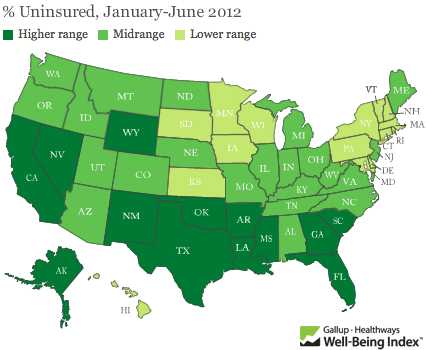
\includegraphics[width=0.9\textwidth]{3-1_define_probability/figures/uninsured}
}

\ct{ \webURL{http://www.gallup.com/poll/156851/uninsured-rate-stable-across-states-far-2012.aspx}}

\end{frame}

%%%%%%%%%%%%%%%%%%%%%%%%%%%%%%%%%%%%

\subsection{Recap}

%%%%%%%%%%%%%%%%%%%%%%%%%%%%%%%%%%%%

\begin{frame}
\frametitle{Disjoint vs. complementary}

\dq{Do the sum of probabilities of two disjoint events always add up to 1?}

\pause

\soln{Not necessarily, there may be more than 2 events in the sample space, e.g. party affiliation.}

\pause
$\:$ \\

\dq{Do the sum of probabilities of two complementary events always add up to 1?}

\pause

\soln{Yes, that's the definition of complementary, e.g. heads and tails. }

\end{frame}

%%%%%%%%%%%%%%%%%%%%%%%%%%%%%%%%%%%%

\begin{frame}
\frametitle{Putting everything together...}

\dq{If we were to randomly select 5 Texans, what is the probability that at least one is uninsured?}

\begin{itemize}

\item If we were to randomly select 5 Texans, the sample space for the number of Texans who are uninsured would be:
\[ S = \{0, 1, 2, 3, 4, 5\} \]

\item We are interested in instances where at least one person is uninsured:
\[ S = \{0, \orange{$1, 2, 3, 4, 5$} \} \]

\item So we can divide up the sample space into two categories:
\[ S = \{0, \orange{at~least~one} \} \]

\end{itemize}

\end{frame}

%%%%%%%%%%%%%%%%%%%%%%%%%%%%%%%%%%%%

\begin{frame}
\frametitle{Putting everything together...}

Since the probability of the sample space must add up to 1:
\begin{eqnarray*}
Prob(at~least~1~uninsured) &=& 1 - Prob(none~uninsured) \\
\pause
&=& 1 - [(1-0.255)^5] \\
\pause
&=& 1- 0.745^5 \\
\pause
&=& 1 - 0.23 \\
\pause
&=& 0.77
\end{eqnarray*}

$\:$ \\
$\:$ \\

\formula{At least 1}{\[P(at~least~one) = 1 - P(none)\]}

\end{frame}

%%%%%%%%%%%%%%%%%%%%%%%%%%%%%%%%%%%%

\begin{frame}
\frametitle{Practice}

\pq{Roughly 20\% of undergraduates at a university are vegetarian or vegan. What is the probability that, among a random sample of 3 undergraduates, at least one is vegetarian or vegan?}

\twocol{0.3}{0.6}{
\begin{enumerate}[(a)]
\item $1 - 0.2 \times 3$
\item $1 - 0.2^3$
\item $0.8^3$
\item $1 - 0.8 \times 3$
\solnMult{$1 - 0.8^3$}
\end{enumerate}
}
{
\soln{ \only<2>{
$P(at~least~1~from~veg) = 1- P(none~veg)$ \\
$= 1 - (1 - 0.2)^3$ \\
$= 1 - 0.8^3$ \\
$= 1 - 0.512 = 0.488$ }}
}

\end{frame}

%%%%%%%%%%%%%%%%%%%%%%%%%%%%%%%%%%%%
%%%%%%%%%%%%%%%%%%%%%%%%%%%%%%%%%%%%

\section{Conditional probability}

%%%%%%%%%%%%%%%%%%%%%%%%%%%%%%%%%%%%

\subsection{Exploring probabilities with a contingency table}

%%%%%%%%%%%%%%%%%%%%%%%%%%%%%%%%%%%%

\begin{frame}
\frametitle{Relapse}

Researchers randomly assigned 72 chronic users of cocaine into three groups: desipramine (antidepressant), lithium (standard treatment for cocaine) and placebo. Results of the study are summarized below.

{\small
\begin{center}
\begin{tabular}{l | c c | c}
			& 		& no 		&  \\
			& relapse	& relapse	& total \\
\hline
desipramine	& 10		& 14		& 24 \\
lithium		& 18		& 6		& 24 \\
placebo		& 20		& 4		& 24 \\
\hline
total			& 48		& 24		& 72
\end{tabular}
\end{center}
}

\ct{\webURL{http://www.oswego.edu/~srp/stats/2_way_tbl_1.htm}}

\end{frame}

%%%%%%%%%%%%%%%%%%%%%%%%%%%%%%%%%%%%

\begin{frame}

\dq{What is the probability that a patient did not relapse?}


{\small
\begin{center}
\begin{tabular}{l | c c | c}
			& 		& no 		&  \\
			& relapse	& relapse	& total \\
\hline
desipramine	& 10		& 14		& 24 \\
lithium		& 18		& 6		& 24 \\
placebo		& 20		& 4		& 24 \\
\hline
total			& 48		& 24		& 72
\end{tabular}
\end{center}
}

\end{frame}

%%%%%%%%%%%%%%%%%%%%%%%%%%%%%%%%%%%%

\subsection{Marginal and joint probabilities}

%%%%%%%%%%%%%%%%%%%%%%%%%%%%%%%%%%%%

\begin{frame}
\frametitle{Marginal probability}

\dq{What is the probability that a patient relapsed?}

{\small
\begin{center}
\begin{tabular}{l | c c | c}
			& 		& no 		&  \\
			& relapse	& relapse	& total \\
\hline
desipramine	& 10		& 14		& 24 \\
lithium		& 18		& 6		& 24 \\
placebo		& 20		& 4		& 24 \\
\hline
total			& \only<1>{48}\only<2->{\red{48}}		& 24		&  \only<1>{72}\only<2->{\red{72}}
\end{tabular}
\end{center}
}

\onslide<2->{P(relapsed) = $\frac{48}{72} \approx 0.67$} \\

\end{frame}

%%%%%%%%%%%%%%%%%%%%%%%%%%%%%%%%%%%%

\begin{frame}
\frametitle{Joint probability}

\dq{What is the probability that a patient received the antidepressant (desipramine) \underline{and} relapsed?}

{\small
\begin{center}
\begin{tabular}{l | c c | c}
			& 		& no 		&  \\
			& relapse	& relapse	& total \\
\hline
desipramine	& \only<1>{10} \only<2->{\red{10}}		& 14		& 24 \\
lithium		& 18		& 6		& 24 \\
placebo		& 20		& 4		& 24 \\
\hline
total			& 48	& 24		&  \only<1>{72} \only<2->{\red{72}}
\end{tabular}
\end{center}
}

\onslide<2->{P(relapsed and desipramine) = $\frac{10}{72} \approx 0.14$} \\

\end{frame}

%%%%%%%%%%%%%%%%%%%%%%%%%%%%%%%%%%%%

\subsection{Defining conditional probability}

%%%%%%%%%%%%%%%%%%%%%%%%%%%%%%%%%%%%

\begin{frame}
\frametitle{Conditional probability}

\formula{Conditional probability}{
The conditional probability of the outcome of interest $A$ given condition $B$ is calculated as
\[ P(A|B) = \frac{P(A~and~B)}{P(B)} \]
}

\pause

\twocol{0.5}{0.5}
{
{\small
\begin{center}
\begin{tabular}{l | c c | c}
			& 		& no 		&  \\
			& relapse	& relapse	& total \\
\hline
desipramine	& 10		& 14		& 24 \\
lithium		& 18		& 6		& 24 \\
placebo		& 20		& 4		& 24  \\
\hline
total			& 48		& 24		&  72
\end{tabular}
\end{center}
}
}
{
\begin{eqnarray*}
&&P(relapse |  desipramine) \\
&&= \frac{P(relapse ~ and ~ desipramine)}{P(desipramine)} \\
\pause
&&= \frac{10 / 72}{24 / 72} \\
\pause
&&= \frac{10}{24} \\
\pause
&&= 0.42
\end{eqnarray*}
}

\end{frame}

%%%%%%%%%%%%%%%%%%%%%%%%%%%%%%%%%%%%

\begin{frame}
\frametitle{Conditional probability (cont.)}

\dq{If we know that a patient received the antidepressant (desipramine), what is the probability that they relapsed?}

{\small
\begin{center}
\begin{tabular}{l | c c | c}
			& 		& no 		&  \\
			& relapse	& relapse	& total \\
\hline
\rowcolor[gray]{.7}
desipramine	& \only<1>{10} \only<2->{\red{10}}			& 14		& \only<1>{24} \only<2->{\red{24}} \\
lithium		& 18		& 6		& 24 \\
placebo		& 20 		& 4		& 24  \\
\hline
total			& 48	& 24		&  72
\end{tabular}
\end{center}
}

\onslide<2->{P(relapse $|$  desipramine) = $\frac{10}{24} \approx 0.42$} \\

\onslide<3->{
$\:$ \\
P(relapse $|$  lithium) = $\frac{18}{24} \approx 0.75$ \\
P(relapse $|$  placebo) = $\frac{20}{24} \approx 0.83$ \\
}

\end{frame}

%%%%%%%%%%%%%%%%%%%%%%%%%%%%%%%%%%%%

\begin{frame}
\frametitle{Conditional probability (cont.)}

\dq{If we know that a patient relapsed, what is the probability that they received the antidepressant (desipramine)?}

{\small
\begin{center}
\begin{tabular}{l | >{\columncolor[gray]{0.7}[0pt]}c c | c}
			& 		& no 		&  \\
			& relapse	& relapse	& total \\
\hline
desipramine	& \only<1>{10} \only<2->{\red{10}}			& 14		& 24 \\
lithium		& 18		& 6		& 24 \\
placebo		& 20		& 4		& 24  \\
\hline
total			& \only<1>{48} \only<2->{\red{48}}	& 24		&  72
\end{tabular}
\end{center}
}

\onslide<2->{P(desipramine $|$  relapse) = $\frac{10}{48} \approx 0.21$} \\

\onslide<3->{
$\:$ \\
P(lithium $|$  relapse) = $\frac{18}{48} \approx 0.375$ \\
P(placebo $|$  relapse) = $\frac{20}{48} \approx 0.42$ \\
}

\end{frame}

%%%%%%%%%%%%%%%%%%%%%%%%%%%%%%%%%%%%

\subsection{General multiplication rule}

%%%%%%%%%%%%%%%%%%%%%%%%%%%%%%%%%%%%

\begin{frame}
\frametitle{General multiplication rule}

\begin{itemize}

\item Earlier we saw that if two events are independent, their joint probability is simply the product of their probabilities. If the events are not believed to be independent, the joint probability is calculated slightly differently.

\pause

\item If $A$ and $B$ represent two outcomes or events, then
\formula{\[ P(A~and~B) = P(A|B) \times P(B) \]}
Note that this formula is simply the conditional probability formula, rearranged.
\pause

\item It is useful to think of $A$ as the outcome of interest and $B$ as the condition.

\end{itemize}

\end{frame}

%%%%%%%%%%%%%%%%%%%%%%%%%%%%%%%%%%%%

\subsection{Independence considerations in conditional probability}

%%%%%%%%%%%%%%%%%%%%%%%%%%%%%%%%%%%%

\begin{frame}
\frametitle{Independence and conditional probabilities}

Consider the following (hypothetical) distribution of gender and major of students in an introductory statistics class:

{\small
\begin{center}
\begin{tabular}{l | c c | c}
			& social	& non-social 		&  \\
			& science	& science	& total \\
\hline
female		& 30		& 20		& 50 \\
male			& 30		& 20		& 50 \\
\hline
total			& 60		& 40		& 100
\end{tabular}
\end{center}
}

\pause

\begin{itemize}

\item The probability that a randomly selected student is a social science major is \pause $\frac{60}{100} = 0.6$. 

\pause

\item The probability that a randomly selected student is a social science major given that they are female is \pause $\frac{30}{50} = 0.6$. 

\pause

\item Since $P(SS | M)$ also equals 0.6, major of students in this class does not depend on their gender: P(SS $|$ F) = P(SS).

\end{itemize}

\end{frame}

%%%%%%%%%%%%%%%%%%%%%%%%%%%%%%%%%%%%

\begin{frame}
\frametitle{Independence and conditional probabilities (cont.)}

Generically, if $P(A|B) = P(A)$ then the events $A$ and $B$ are said to be independent.

\pause

\begin{itemize}

\item Conceptually: Giving $B$ doesn't tell us anything about $A$.

\pause

\item Mathematically: We know that if events $A$ and $B$ are independent, $P(A~and~B) = P(A) \times P(B)$. Then,
\[ P(A|B) = \frac{P(A~and~B)}{P(B)} = \frac{P(A) \times P(B)}{P(B)} = P(A) \]

\end{itemize}

\end{frame}

%%%%%%%%%%%%%%%%%%%%%%%%%%%%%%%%%%%%

\subsection{Tree diagrams}

%%%%%%%%%%%%%%%%%%%%%%%%%%%%%%%%%%%%

\begin{frame}
\frametitle{Breast cancer screening}

\begin{itemize}

\item American Cancer Society estimates that about 1.7\% of women have breast cancer. \\
{\small\webURL{http://www.cancer.org/cancer/cancerbasics/cancer-prevalence}}

\item Susan G. Komen For The Cure Foundation states that mammography correctly identifies about 78\% of women who truly have breast cancer. \\
{\small\webURL{http://ww5.komen.org/BreastCancer/AccuracyofMammograms.html}}

\item An article published in 2003 suggests that up to 10\% of all mammograms result in false positives for patients who do not have cancer. \\{\small \webURL{http://www.ncbi.nlm.nih.gov/pmc/articles/PMC1360940}}

\end{itemize}

\vfill

\Note{These percentages are approximate, and very difficult to estimate.}

\end{frame}

%%%%%%%%%%%%%%%%%%%%%%%%%%%%%%%%%%%

\begin{frame}
\frametitle{Inverting probabilities}

\dq{When a patient goes through breast cancer screening there are two competing claims: patient had cancer and patient doesn't have cancer. If a mammogram yields a positive result, what is the probability that patient actually has cancer?}

\pause

\twocol{0.7}{0.3}{
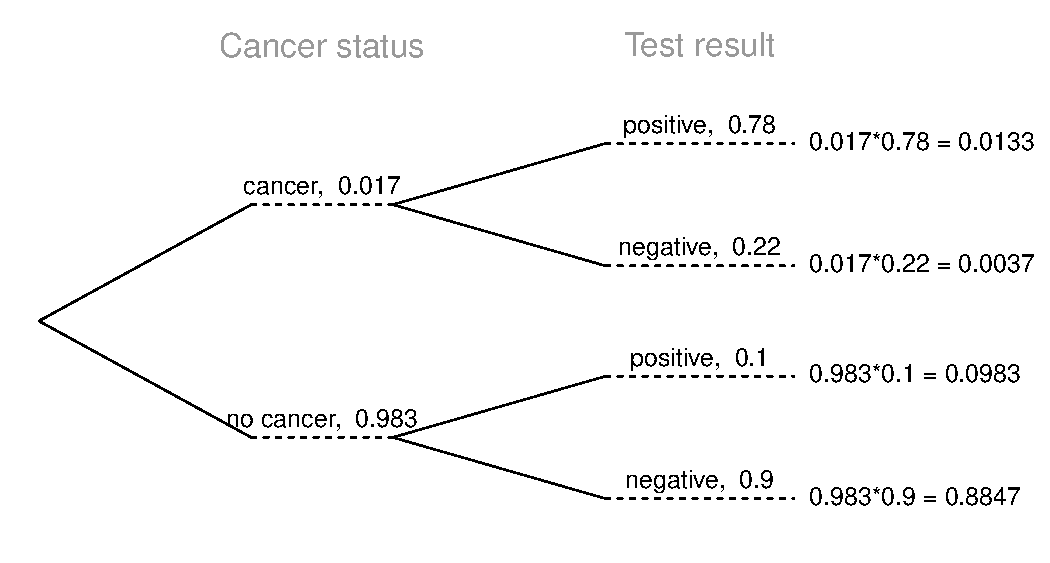
\includegraphics[width=\textwidth]{3-2_conditional_probability/figures/cancer_tree/cancer_tree_first} 
}
{
\pause
{\footnotesize
\begin{eqnarray*}
&&P(C | +) \\
\pause
&&= \frac{P(C~and~+)}{P(+)} \\
\pause
&&= \frac{0.0133}{0.0133 + 0.0983} \\
\pause
&&= 0.12
\end{eqnarray*}
}
}

\pause

\Note{Tree diagrams are useful for inverting probabilities: we are given $P(+|C)$ and asked for $P(C|+)$.}

\end{frame}

%%%%%%%%%%%%%%%%%%%%%%%%%%%%%%%%%%%

\begin{frame}
\frametitle{Practice}

\pq{Suppose a woman who gets tested once and obtains a positive result wants to get tested again. In the second test, what should we assume to be the probability of this specific woman having cancer?}

\begin{enumerate}[(a)]
\item 0.017
\solnMult{0.12}
\item 0.0133
\item 0.88
\end{enumerate}

\end{frame}

%%%%%%%%%%%%%%%%%%%%%%%%%%%%%%%%%%%

\begin{frame}
\frametitle{Practice}

\pq{What is the probability that this woman has cancer if this second mammogram also yielded a positive result?}

\twocol{0.2}{0.7}
{
\begin{enumerate}[(a)]
\item 0.0936
\item 0.088
\item 0.48
\solnMult{0.52}
\end{enumerate}
}
{
\solnGr{\only<2->{
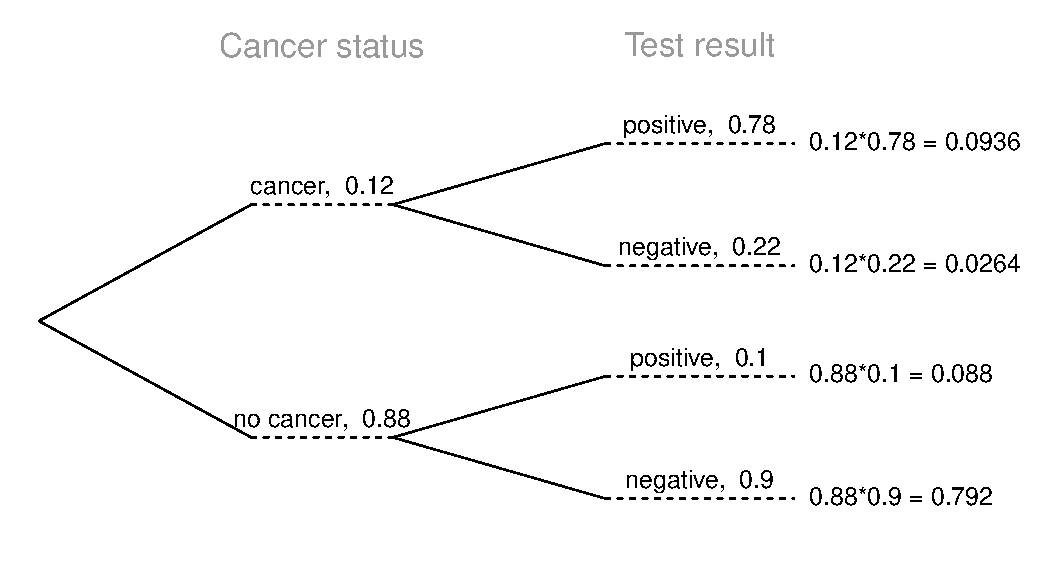
\includegraphics[width=\textwidth]{3-2_conditional_probability/figures/cancer_tree/cancer_tree_second} 
}}
}

\soln{\only<3->{
{\small \[P(C | +) = \frac{P(C~and~+)}{P(+)} = \frac{0.0936}{0.0936+0.088} = 0.52\]}
}}

\end{frame}

%%%%%%%%%%%%%%%%%%%%%%%%%%%%%%%%%%%

\subsection{Bayes' Theorem}

%%%%%%%%%%%%%%%%%%%%%%%%%%%%%%%%%%%%

\begin{frame}
\frametitle{Bayes' Theorem}

\begin{itemize}

\item The conditional probability formula we have seen so far is a special case of the Bayes' Theorem, which is applicable even when events have more than just two outcomes.

\pause 

\item \hl{Bayes' Theorem:}
\formula{
\[ P(outcome~A_1~of~variable~1~|~outcome~B~of~variable~2) \]
\[ = \frac{P(B|A_1)P(A_1)}{P(B|A_1)P(A_1) + P(B|A_2)P(A_2) + \cdots + P(B|A_k)P(A_k)} \]
}
where $A_2$, $\cdots$, $A_k$ represent all other possible outcomes of variable 1.

\end{itemize}

\end{frame}

%%%%%%%%%%%%%%%%%%%%%%%%%%%%%%%%%%%

\begin{frame}
\frametitle{Application activity: Inverting probabilities}

\app{{\footnotesize A common epidemiological model for the spread of diseases is the SIR model, where the population is partitioned into three groups: Susceptible, Infected, and Recovered. This is a reasonable model for diseases like chickenpox where a single infection usually provides immunity to subsequent infections. Sometimes these diseases can also be difficult to detect. \vspace{2mm} \\
Imagine a population in the midst of an epidemic where 60\% of the population is considered susceptible, 10\% is infected, and 30\% is recovered. The only test for the disease is accurate 95\% of the time for susceptible individuals, 99\% for infected individuals, but 65\% for recovered individuals. (Note: In this case accurate means returning a negative result for susceptible and recovered individuals and a positive result for infected individuals). \vspace{2mm} \\
Draw a probability tree to reflect the information given above. If the individual has tested positive, what is the probability that they are actually infected?
}}

\end{frame}

%%%%%%%%%%%%%%%%%%%%%%%%%%%%%%%%%%%

\begin{frame}
\frametitle{Application activity: Inverting probabilities (cont.)}

\vspace{-0.5cm}

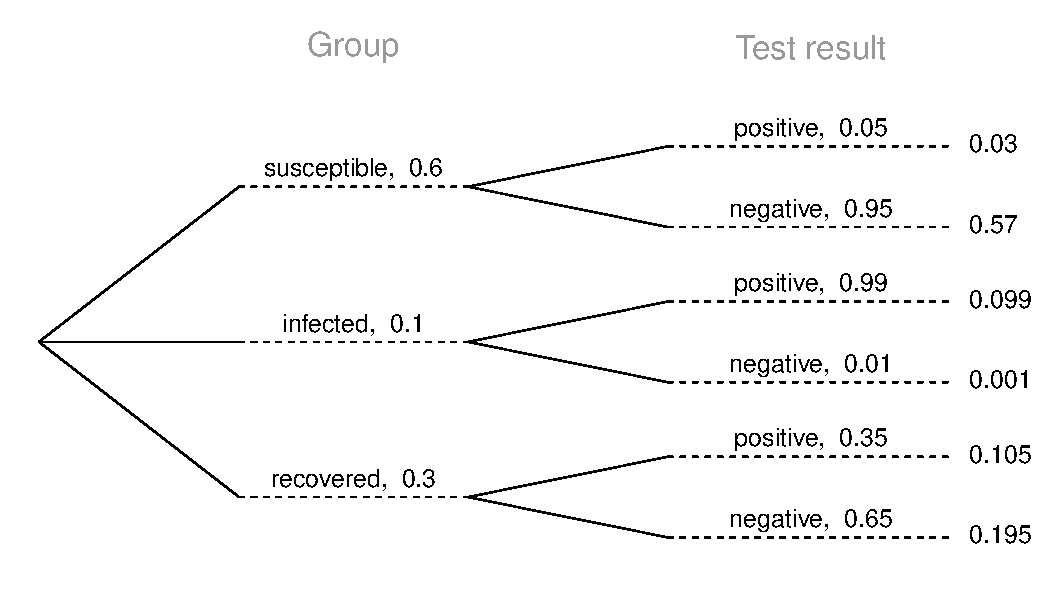
\includegraphics[width=\textwidth]{3-2_conditional_probability/figures/sir_tree/sir_tree} 

\pause

\[ P(inf | +) = \frac{P(inf~and~+)}{P(+)} = \frac{0.099}{0.03 + 0.099 + 0.105} \approx 0.423 \]


\end{frame}

%%%%%%%%%%%%%%%%%%%%%%%%%%%%%%%%%%%%
%
%\end{frame}
%%%%%%%%%%%%%%%%%%%%%%%%%%%%%%%%%%%%

\section{Sampling from a small population}

%%%%%%%%%%%%%%%%%%%%%%%%%%%%%%%%%%%%

\begin{frame}
\frametitle{Sampling with replacement}

When sampling \hl{with replacement}, you put back what you just drew.

\pause

\begin{itemize}

\item Imagine you have a bag with 5 red, 3 blue and 2 orange chips in it. What is the probability that the first chip you draw is blue?
\begin{center}
5 \textcolor{red}{$\CIRCLE$}~, 3 \textcolor{blue}{$\CIRCLE$}~, 2 \textcolor{orange}{$\CIRCLE$}
\end{center}

\pause

\[ Prob(1^{st} \text{ chip } B) = \frac{3}{5 + 3 + 2} = \frac{3}{10} = 0.3 \]

\pause

\item Suppose you did indeed pull a blue chip in the first draw. If drawing with replacement, what is the probability of drawing a blue chip in the second draw?

\pause

\begin{center}
$1^{st}$ draw: 5 \textcolor{red}{$\CIRCLE$}~, 3 \textcolor{blue}{$\CIRCLE$}~, 2 \textcolor{orange}{$\CIRCLE$} \\

\pause

$2^{nd}$ draw: 5 \textcolor{red}{$\CIRCLE$}~, 3 \textcolor{blue}{$\CIRCLE$}~, 2 \textcolor{orange}{$\CIRCLE$}
\end{center}

\pause

\[ Prob(2^{nd} \text{ chip } B | 1^{st} \text{ chip } B) = \frac{3}{10} = 0.3 \]

\end{itemize}

\end{frame}

%%%%%%%%%%%%%%%%%%%%%%%%%%%%%%%%%%%%%

\begin{frame}
\frametitle{Sampling with replacement (cont.)}

\begin{itemize}

\item Suppose you actually pulled an orange chip in the first draw. If drawing with replacement, what is the probability of drawing a blue chip in the second draw?

\pause

\begin{center}
$1^{st}$ draw: 5 \textcolor{red}{$\CIRCLE$}~, 3 \textcolor{blue}{$\CIRCLE$}~, 2 \textcolor{orange}{$\CIRCLE$} \\
\pause
$2^{nd}$ draw: 5 \textcolor{red}{$\CIRCLE$}~, 3 \textcolor{blue}{$\CIRCLE$}~, 2 \textcolor{orange}{$\CIRCLE$}
\end{center}
\pause
\[ Prob(2^{nd} \text{ chip } B | 1^{st} \text{ chip } O) = \frac{3}{10} = 0.3 \]

\pause
\item If drawing with replacement, what is the probability of drawing two blue chips in a row?
\begin{center}

\pause
$1^{st}$ draw: 5 \textcolor{red}{$\CIRCLE$}~, 3 \textcolor{blue}{$\CIRCLE$}~, 2 \textcolor{orange}{$\CIRCLE$} \\
$2^{nd}$ draw: 5 \textcolor{red}{$\CIRCLE$}~, 3 \textcolor{blue}{$\CIRCLE$}~, 2 \textcolor{orange}{$\CIRCLE$}
\end{center}
\pause
\[ Prob(1^{st} \text{ chip } B) \cdot Prob(2^{nd} \text{ chip } B | 1^{st} \text{ chip } B) = 0.3 \times 0.3 \]
\[ = 0.3^2 = 0.09 \]

\end{itemize}

\end{frame}

%%%%%%%%%%%%%%%%%%%%%%%%%%%%%%%%%%%%%

\begin{frame}
\frametitle{Sampling with replacement (cont.)}

\begin{itemize}

\item When drawing with replacement, probability of the second chip being blue does not depend on the color of the first chip since whatever we draw in the first draw gets put back in the bag.
\[ Prob(B | B) = Prob(B | O) \]

\item In addition, this probability is equal to the probability of drawing a blue chip in the first draw, since the composition of the bag never changes when sampling with replacement.
\[ Prob(B | B) = Prob(B) \]

\item \hl{When drawing with replacement, draws are independent.}

\end{itemize}

\end{frame}


%%%%%%%%%%%%%%%%%%%%%%%%%%%%%%%%%%%%%

\begin{frame}
\frametitle{Sampling without replacement}

When drawing \hl{without replacement} you do not put back what you just drew.

\begin{itemize}

\pause

\item Suppose you pulled a blue chip in the first draw. If drawing without replacement, what is the probability of drawing a blue chip in the second draw?
\pause
\begin{center}
$1^{st}$ draw: 5 \textcolor{red}{$\CIRCLE$}~, 3 \textcolor{blue}{$\CIRCLE$}~, 2 \textcolor{orange}{$\CIRCLE$} \\
\pause
$2^{nd}$ draw: 5 \textcolor{red}{$\CIRCLE$}~, 2 \textcolor{blue}{$\CIRCLE$}~, 2 \textcolor{orange}{$\CIRCLE$}
\end{center}
\pause
\[ Prob(2^{nd} \text{ chip } B | 1^{st} \text{ chip } B) = \frac{2}{9} = 0.22 \]

\pause

\item If drawing without replacement, what is the probability of drawing two blue chips in a row?
\begin{center}

\pause
$1^{st}$ draw: 5 \textcolor{red}{$\CIRCLE$}~, 3 \textcolor{blue}{$\CIRCLE$}~, 2 \textcolor{orange}{$\CIRCLE$} \\
$2^{nd}$ draw: 5 \textcolor{red}{$\CIRCLE$}~, 2 \textcolor{blue}{$\CIRCLE$}~, 2 \textcolor{orange}{$\CIRCLE$}
\end{center}
\pause
\[ Prob(1^{st} \text{ chip } B) \cdot Prob(2^{nd} \text{ chip } B | 1^{st} \text{ chip } B)  = 0.3 \times 0.22 \]
\[ = 0.066 \]

\end{itemize}

\end{frame}

%%%%%%%%%%%%%%%%%%%%%%%%%%%%%%%%%%%%%

\begin{frame}
\frametitle{Sampling without replacement (cont.)}

\begin{itemize}

\item When drawing without replacement, the probability of the second chip being blue given the first was blue is not equal to the probability of drawing a blue chip in the first draw since the composition of the bag changes with the outcome of the first draw.
\[ Prob(B | B) \ne Prob(B) \]

\pause

\item \hl{When drawing without replacement, draws are not independent.}

\pause

\item This is especially important to take note of when the sample sizes are small. If we were dealing with, say, 10,000 chips in a (giant) bag, taking out one chip of any color would not have as big an impact on the probabilities in the second draw.

\end{itemize}

\end{frame}

%%%%%%%%%%%%%%%%%%%%%%%%%%%%%%%%%%%%%

\begin{frame}
\frametitle{Practice}

\pq{In most card games cards are dealt without replacement. What is the probability of being dealt an ace and then a 3? Choose the closest answer.}

\twocol{0.3}{0.6}{
\begin{enumerate}[(a)]
\item 0.0045
\item 0.0059
\solnMult{0.0060}
\item 0.1553
\end{enumerate}
}
{
\soln{
\pause
\[ P(ace~then~3) = \frac{4}{52} \times \frac{4}{51} \approx 0.0060 \]
}}

\end{frame}

%%%%%%%%%%%%%%%%%%%%%%%%%%%%%%%%%%%%%
%%%%%%%%%%%%%%%%%%%%%%%%%%%%%%%%%%%%

\section{Random variables}

%%%%%%%%%%%%%%%%%%%%%%%%%%%%%%%%%%%%

\begin{frame}
\frametitle{Random variables}

\begin{itemize}

\item A \hl{random variable} is a numeric quantity whose value depends on the outcome of a random event
\begin{itemize}
\item We use a capital letter, like $X$, to denote a random variable
\item The values of a random variable are denoted with a lowercase letter, in this case $x$
\item For example, $P(X = x)$
\end{itemize}

\item There are two types of random variables:
\begin{itemize}
\item \hl{Discrete random variables} often take only integer values
\begin{itemize}
\item Example: Number of credit hours, Difference in number of credit hours this term vs last
\end{itemize}
\item \hl{Continuous random variables} take real (decimal) values
\begin{itemize}
\item Example: Cost of books this term, Difference in cost of books this term vs last
\end{itemize}
\end{itemize}

\end{itemize}

\end{frame}

%%%%%%%%%%%%%%%%%%%%%%%%%%%%%%%%%%%%

\subsection{Expectation}

%%%%%%%%%%%%%%%%%%%%%%%%%%%%%%%%%%%%

\begin{frame}
\frametitle{Expectation}

\begin{itemize}

\item We are often interested in the average outcome of a random variable.

\item We call this the \hl{expected value} (mean), and it is a weighted average of the possible outcomes
\formula{\[\mu = E(X) = \sum_{i = 1}^k x_i ~ P(X = x_i)\]}

\end{itemize}

\end{frame}

%%%%%%%%%%%%%%%%%%%%%%%%%%%%%%%%%%%%

\begin{frame}
\frametitle{Expected value of a discrete random variable}

\dq{In a game of cards you win \$1 if you draw a heart, \$5 if you draw an ace (including the ace of hearts), \$10 if you draw the king of spades and nothing for any other card you draw. Write the probability model for your winnings, and calculate your expected winning.}

\pause

\begin{center}
\renewcommand{\arraystretch}{1.5}
\begin{tabular}{l | c | c | c }
Event		& $X$ 		& $P(X)$        		& $X ~ P(X)$ \\
\hline
Heart (not ace)	& $1$		& $\frac{12}{52}$	& $\frac{12}{52}$ \\
Ace			& $5$		& $\frac{4}{52}$	& $\frac{20}{52}$ \\	
King of spades	& $10$		& $\frac{1}{52}$	& $\frac{10}{52}$ \\	
All else		& $0$		& $\frac{35}{52}$	& $0$ \\
\hline
Total			&			&				& $E(X) = \frac{42}{52} \approx 0.81$
\end{tabular}

\end{center}

\end{frame}

%%%%%%%%%%%%%%%%%%%%%%%%%%%%%%%%%%%%

\begin{frame}
\frametitle{Expected value of a discrete random variable (cont.)}

Below is a visual representation of the probability distribution of winnings from this game:

\begin{center}
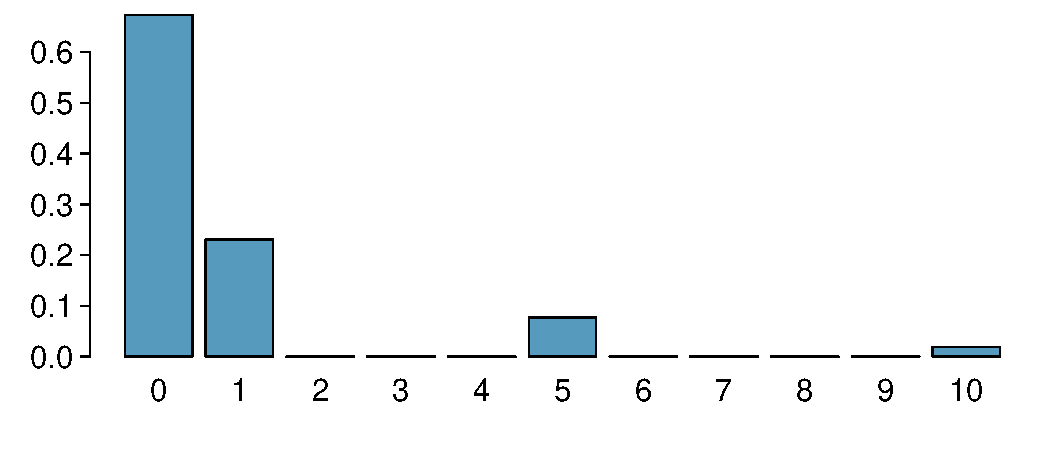
\includegraphics[width=0.8\textwidth]{3-4_random_variables/figures/card_game/card_game}
\end{center}

\end{frame}

%%%%%%%%%%%%%%%%%%%%%%%%%%%%%%%%%%%%

\subsection{Variability in random variables}

%%%%%%%%%%%%%%%%%%%%%%%%%%%%%%%%%%%%

\begin{frame}
\frametitle{Variability}

We are also often interested in the variability in the values of a random variable.

\formula{
\[ \sigma^2 = Var(X) = \sum_{i = 1}^k (x_i - E(X))^2 P(X = x_i) \]
\[ \sigma = SD(X) = \sqrt{Var(X)} \]
}

\end{frame}

%%%%%%%%%%%%%%%%%%%%%%%%%%%%%%%%%%%%

\begin{frame}
\frametitle{Variability of a discrete random variable}

\dq{For the previous card game example, how much would you expect the winnings to vary from game to game?}

\vspace{2mm}
\only<2->{
{\footnotesize
\begin{center}
\renewcommand{\arraystretch}{2}
\begin{tabular}{c | c | c | l | p{4cm}}
$X$ & $P(X)$         & $X ~ P(X)$      & \multicolumn{1}{c|}{$(X - E(X))^2$}  & \multicolumn{1}{c}{$P(X) ~ (X - E(X))^2$}  \\
\hline
1 & $\frac{12}{52}$  & $1 \times \frac{12}{52} = \frac{12}{52}$ & $(1 - 0.81)^2 = 0.0361$ &  $\frac{12}{52} \times 0.0361 = 0.0083$ \\
\hline
5 & $\frac{4}{52}$   & $5 \times \frac{4}{52} = \frac{20}{52}$ & $(5 - 0.81)^2 = 17.5561$  & $\frac{4}{52} \times 17.5561 = 1.3505$ \\
\hline
10  & $\frac{1}{52}$ & $10 \times \frac{1}{52} = \frac{10}{52}$  & $(10 - 0.81)^2 = 84.4561$   & $\frac{1}{52} \times 84.0889 = 1.6242$ \\
\hline
0 & $\frac{35}{52}$  & $0 \times \frac{35}{52} = 0$  & $(0 - 0.81)^2 = 0.6561$ & $\frac{35}{52} \times 0.6561 = 0.4416$ \\
\hline
  &       & $E(X) = 0.81$ & & \soln{\only<3->{$V(X) = 3.4246$}} \\
 &       &                                                         & & \soln{\only<4>{$SD(X) = \sqrt{3.4246} = 1.85$}} \\
\end{tabular}
\end{center}
}
}
\end{frame}

%%%%%%%%%%%%%%%%%%%%%%%%%%%%%%%%%%%%

\subsection{Linear combinations of random variables}

%%%%%%%%%%%%%%%%%%%%%%%%%%%%%%%%%%%%

\begin{frame}
\frametitle{Linear combinations}

\begin{itemize}

\item A \hl{linear combination} of random variables $X$ and $Y$ is given by

\[ aX + bY \]

where $a$ and $b$ are some fixed numbers.

\pause

\item The average value of a linear combination of random variables is given by
\formula{\[ E(aX + bY) = a \times E(X) + b \times E(Y) \]}

\end{itemize}

\end{frame}

%%%%%%%%%%%%%%%%%%%%%%%%%%%%%%%%%%%%

\begin{frame}
\frametitle{Calculating the expectation of a linear combination}

\dq{On average you take 10 minutes for each statistics homework problem and 15 minutes for each chemistry homework problem. This week you have 5 statistics and 4 chemistry homework problems assigned. What is the total time you expect to spend on statistics and chemistry homework for the week?}

\soln{
\pause
\begin{align*} 
E(S + S + S + S + S + C + C + C + C) &= 5 \times E(S) + 4 \times E(C) \\
&= 5 \times 10 + 4 \times 15 \\
&= 50 + 60 \\
&= 110~min 
\end{align*}
}

\end{frame}

%%%%%%%%%%%%%%%%%%%%%%%%%%%%%%%%%%%%

\subsection{Variability in linear combinations of random variables}

%%%%%%%%%%%%%%%%%%%%%%%%%%%%%%%%%%%%

\begin{frame}
\frametitle{Linear combinations}

\begin{itemize}

\item The variability of a linear combination of two independent random variables is calculated as
\formula{\[ V(aX + bY) = a^2 \times V(X) + b^2 \times V(Y) \]}

\pause 

\item The standard deviation of the linear combination is the square root of the variance.

\end{itemize}

\pause 
\vfill

\Note{If the random variables are not independent, the variance calculation gets a little more complicated and is beyond the scope of this course.}

\end{frame}

%%%%%%%%%%%%%%%%%%%%%%%%%%%%%%%%%%%%

\begin{frame}
\frametitle{Calculating the variance of a linear combination}

\dq{The standard deviation of the time you take for each statistics homework problem is 1.5 minutes, and it is 2 minutes for each chemistry problem. What is the standard deviation of the time you expect to spend on statistics and physics homework for the week if you have 5 statistics and 4 chemistry homework problems assigned? Suppose that the time it takes to complete each problem is independent of another.}

\soln{
\pause
\begin{align*} 
V(S + S + S + S + S + C + C + C + C) &= V(S) + V(S) + V(S) + V(S) + V(S) + V(C) + V(C) + V(C) + V(C) \\
&= 5 \times V(S) + 4 \times V(C) \\
&= 5 \times 1.5^2 + 4 \times 2^2 \\
&= 27.25
\end{align*}
}

\end{frame}

%%%%%%%%%%%%%%%%%%%%%%%%%%%%%%%%%%%%

\subsection{Recap}

%%%%%%%%%%%%%%%%%%%%%%%%%%%%%%%%%%%%

\begin{frame}
\frametitle{Practice}

\pq{A casino game costs \$5 to play. If the first card you draw is red, then you get to draw a second card (without replacement). If the second card is the ace of clubs, you win \$500. If not, you don't win anything, i.e. lose your \$5. What is your expected profits/losses from playing this game? {\small Remember: profit/loss = winnings - cost.}}

\begin{multicols}{2}
\begin{enumerate}[(a)]
\item A profit of 5\textcent
\solnMult{A loss of 10\textcent}
\item A loss of 25\textcent
\item A loss of 30\textcent
\end{enumerate}
\end{multicols}

\soln{
\only<2>{
{\small
\renewcommand\arraystretch{1.25}
\begin{tabular}{l c c c r}
Event				& Win	& Profit: $X$	& $P(X)$	& $ X \times P(X)$	\\
\hline
\orange{Red}, {A}{$\clubsuit$}		& 500		& 500 - 5 = 495	& $\frac{26}{52} \times \frac{1}{51} = 	0.0098$ & 	 $495 \times 0.0098 = 4.851$ \\
Other	& 0 			& 0 - 5 = -5	& $1 - 0.0098 = 0.9902$ & $-5 \times 0.9902 = -4.951$ \\  
\hline
					&			&			& 			& $E(X) = -0.1$
\end{tabular}
}
}
}

\end{frame}

%%%%%%%%%%%%%%%%%%%%%%%%%%%%%%%%%%%%

\begin{frame}
\frametitle{Fair game}

A \hl{fair} game is defined as a game that costs as much as its expected payout, i.e. expected profit is 0.

\pause

$\:$

\dq{Do you think casino games in Vegas cost more or less than their expected payouts?}

\soln{
\pause
\begin{columns}[c]
\column{0.6\textwidth}
If those games cost less than their expected payouts, it would mean that the casinos would be losing money on average, and hence they wouldn't be able to pay for all this:
\column{0.4\textwidth}
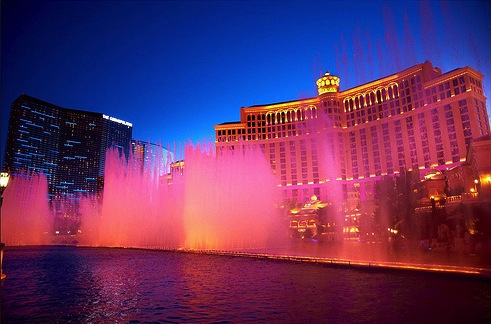
\includegraphics[width=\textwidth]{3-4_random_variables/figures/bellagio.jpg}
\end{columns}
\ct{Image by Moyan\_Brenn on Flickr \webURL{http://www.flickr.com/photos/aigle\_dore/5951714693}.}
}


\end{frame}

%%%%%%%%%%%%%%%%%%%%%%%%%%%%%%%%%%%%%

\begin{frame}
\frametitle{Simplifying random variables}

Random variables do not work like normal algebraic variables:
\[ X + X \ne 2X \]

\pause

{\small
\twocol{0.45}{0.45}
{
\begin{align*}
E(X + X) &= E(X) + E(X) \\
&= 2 E(X) \\
&~  \\
E(2X) &= 2 E(X) \\
&~ 
\end{align*}
}
{
\begin{align*}
Var(X + X) &= Var(X) + Var(X)~{\scriptsize \text{(assuming independence)}} \\
&= 2~Var(X) \\
&~  \\
Var(2X) &= 2^2~Var(X) \\
&= 4~Var(X)
\end{align*}
}
}


\pause

\vspace{3mm}

\mathhl{E(X + X)  = E(2X)}, but \mathhl{Var(X + X) \ne Var(2X)}.

\end{frame}

%%%%%%%%%%%%%%%%%%%%%%%%%%%%%%%%%%%%%

\begin{frame}
\frametitle{Adding or multiplying?}

\dq{A company has 5 Lincoln Town Cars in its fleet. Historical data show that annual maintenance cost for each car is on average \$2,154 with a standard deviation of \$132. What is the mean and the standard deviation of the total annual maintenance cost for this fleet?}

\pause

Note that we have 5 cars each with the given annual maintenance cost $(X_1 + X_2 + X_3 + X_4 + X_5)$, not one car that had 5 times the given annual maintenance cost $(5X)$.

\pause

{\small
\begin{eqnarray*} 
E(X_1 + X_2 + X_3 + X_4 + X_5) &=& E(X_1) + E(X_2) + E(X_3) + E(X_4) + E(X_5) \\
\pause
&=& 5 \times E(X) = 5 \times 2,154 = \$ 10,770 \\
\pause
Var(X_1 + X_2 + X_3 + X_4 + X_5) &=& Var(X_1) + Var(X_2) + Var(X_3) + Var(X_4) + Var(X_5) \\
\pause
&=& 5 \times V(X) = 5 \times 132^2 = \$ 87,120 \\
\pause
SD(X_1 + X_2 + X_3 + X_4 + X_5) &=& \sqrt{87,120} =  295.16
\end{eqnarray*}
}

\end{frame}


%%%%%%%%%%%%%%%%%%%%%%%%%%%%%%%%%%%%

\section{Continuous distributions}

%%%%%%%%%%%%%%%%%%%%%%%%%%%%%%%%%%%%

\begin{frame}
\frametitle{Continuous distributions}

\begin{itemize}

\item Below is a histogram of the distribution of heights of US adults. 

\item The proportion of data that falls in the shaded bins gives the probability that a randomly sampled US adult is between 180 cm and 185 cm (about 5'11" to 6'1").

\end{itemize}

\begin{center}
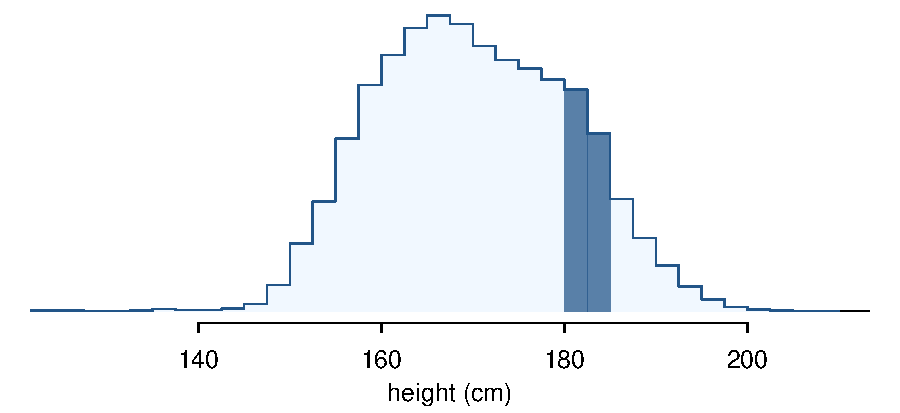
\includegraphics[width=\textwidth]{3-5_continuous_distributions/figures/usHeightsHist180185/usHeightsHist180185}
\end{center}


\end{frame}

%%%%%%%%%%%%%%%%%%%%%%%%%%%%%%%%%%%%

\subsection{From histograms to continuous distributions}

\begin{frame}
\frametitle{From histograms to continuous distributions}

Since height is a continuous numerical variable, its \hl{probability density function} is a smooth curve.

\begin{center}
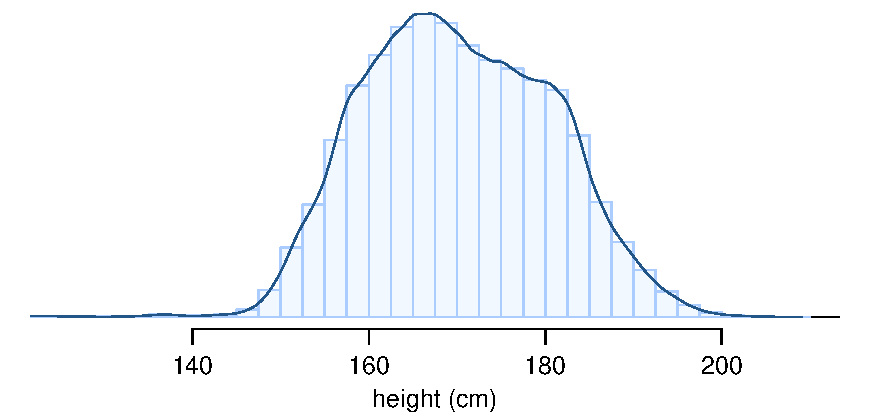
\includegraphics[width=\textwidth]{3-5_continuous_distributions/figures/fdicHeightContDist/fdicHeightContDist}
\end{center}

\end{frame}

%%%%%%%%%%%%%%%%%%%%%%%%%%%%%%%%%%%%

\subsection{Probabilities from continuous distributions}

\begin{frame}
\frametitle{Probabilities from continuous distributions}

Therefore, the probability that a randomly sampled US adult is between 180 cm and 185 cm can also be estimated as the shaded area under the curve.

\begin{center}
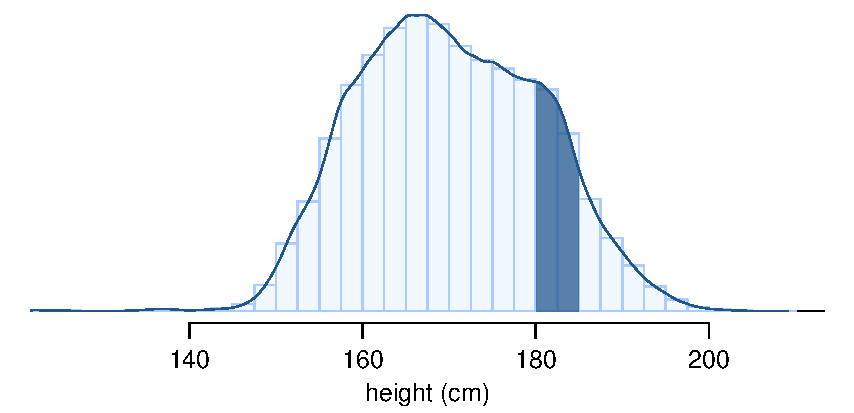
\includegraphics[width=\textwidth]{3-5_continuous_distributions/figures/fdicHeightContDistFilled/fdicHeightContDistFilled}
\end{center}


\end{frame}

%%%%%%%%%%%%%%%%%%%%%%%%%%%%%%%%%%%%

\begin{frame}
\frametitle{By definition...}

Since continuous probabilities are estimated as ``the area under the curve", the probability of a person being exactly 180 cm (or any exact value) is defined as 0.

\begin{center}
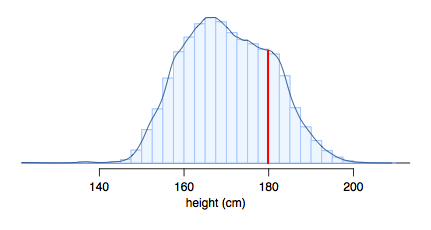
\includegraphics[width=0.8\textwidth]{3-5_continuous_distributions/figures/fdicHeightContDist180}
\end{center}

\end{frame}

%%%%%%%%%%%%%%%%%%%%%%%%%%%%%%%%%%%%


%%%%%%%%%%%%%%%%%%%%%%%%%%%%%%%%%%%%
% End document
%%%%%%%%%%%%%%%%%%%%%%%%%%%%%%%%%%%%

\end{document}